\documentclass{beamer}
\usepackage[ngerman, english]{babel}
\usepackage[latin1]{inputenc}
\usepackage{amsmath,amsfonts,amssymb, graphicx, subfigure}
\usepackage{beamerthemeshadow}
\setbeamercovered{transparent}
\title{\scshape{The EA Ising Model via Parallel Tempering and D-Wave}}
\author{\scshape{Benjamin Krakoff}}

\date{December 3, 2020}


\begin{document}
	\begin{frame}
		\titlepage
	\end{frame}

\begin{frame}{The Edwards Anderson Ising Model}
	Given a graph $G = (V, E)$ with variables $x_i \in \{\pm1\}, i \in V$ and weights $J_{i, j}, (i, j) \in E$, define the hamiltonian
	\begin{align*}
		H(x) = \sum_{(i, j) \in E} J_{i, j} x_ix_j
	\end{align*}

\vspace{30mm}
Finding the global minimum is  an NP-complete optimization problem \cite{1982JPhA...15.3241B}.
	\end{frame}

\begin{frame}{Parallel Tempering: Idea}
	
	\end{frame}

\begin{frame}{Parallel Tempering: Implementation}
	Following \cite{B509983H}
	\begin{itemize}
	\item Start with replicas $x^{(1)}, \ldots, x^{(n)}$ at temperatures $T_1 < \ldots  < T_n$. 
	\item In parallel, run MCMC for each for $n$ steps. 
	\item Choose $i$ at random, swap replicas $x^{(i)}, x^{(i+1)}$ with probability  $\min\{1, e^{(1/T_{i+1}-1/{T_i})(H(x^{(i+1)}) - H(x^{(i)}))}\}$ to satisfy detailed balance for the join probability distribution
	\begin{align*}
		P(x^{(1)}, T_1, \ldots, x^{(n)}, T_n) = \prod_{1\leq i \leq n} P(x^{(i)}, T_i) \propto e^{-\sum_i H(x^{(i)})/T_i}
		\end{align*}
	\end{itemize}
	\end{frame}

\begin{frame}{D-Wave Annealer}
	Consists of a specific sparse graph, Pegasus graph \cite{dattani2019pegasus}. Vertices are sites that can spin up or down, edge couplings can be specified by the user. \\
	\begin{center}
	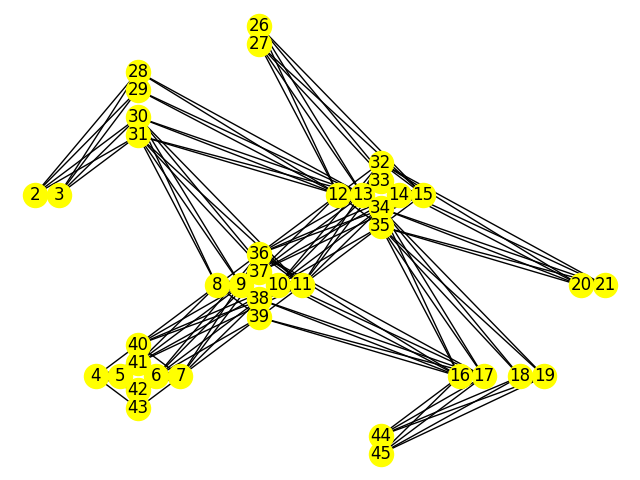
\includegraphics[scale=.3]{Plot.png}
	\end{center}
	D-Wave can minimize arbitrary hamiltonians on subgraphs of Pegasus. To minimize on an arbitrary graph $G$, first need a minor embedding of $G$.
	\end{frame}

\begin{frame}{Minor Embedding: Idea}

	\end{frame}

\begin{frame}{Minor Embedding: D-Wave}
	Minor embedding $G_1$ into $G_2$ is NP-hard, but when $G$ is sparse, smaller than Pegasus there are fast heuristic algorithms \cite{cai2014practical}. When $G$ is not sparse, use a pre-computed minor embedding of complete graph, forget unneeded edges.
\end{frame}

\begin{frame}{Experimental Setup}
	Graphs considered:
	\begin{itemize}
		\item Subgraphs of Pegasus, of size $40$ and $448$ \\
		\item Complete graphs of size $40$ and $119$ (largest possible for D-Wave)
	\end{itemize}
Ensembles considered
\begin{itemize}
 \item $J_{ij} \sim \pm 1$ uniformly
 \item  $J_{ij} \sim \mathcal{N}(0, 1)$.
 \end{itemize} 
Generated 5 hamiltonians for each graph and distribution of $J_{i, j}$ let parallel tempering and D-Wave attempt to solve for the same amount of time.
	\end{frame}

\begin{frame}{Results}
	\begin{figure}
		\centering
		\subfigure{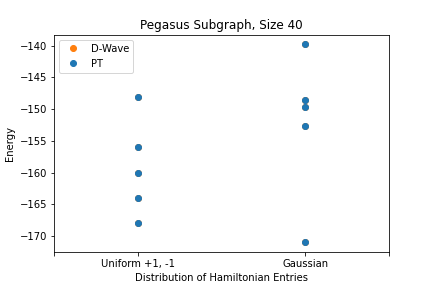
\includegraphics[width=5cm]{pegasus_40.png}} 
		\subfigure{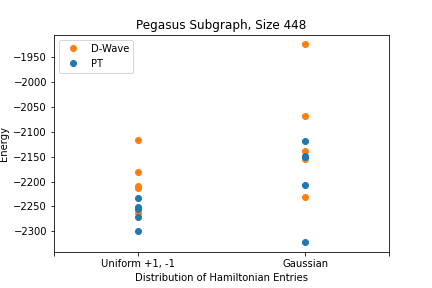
\includegraphics[width=5cm]{pegasus_448.png}} \\
		\subfigure{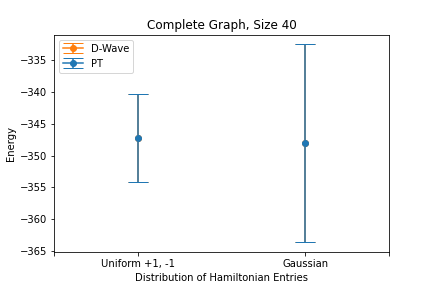
\includegraphics[width=5cm]{clique_40.png}}
		\subfigure{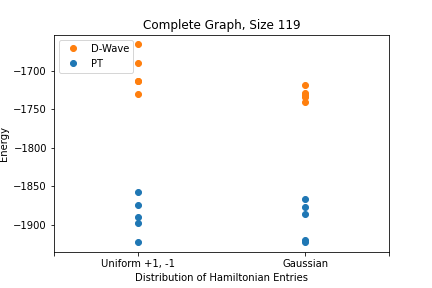
\includegraphics[width=5cm]{clique_119.png}} \\
	\end{figure}

\end{frame}

\begin{frame}{Results}
	\small
	\begin{center}
	\begin{tabular}{c|c|c|c|c}
		& Peg, Uniform & Peg, Gaussian & Cliq, Uniform & Cliq, Gaussian \\
		\hline
		Discrepancy & .446 &   .386 & .074 & .106 \\
	\end{tabular}
\end{center}
\end{frame}

\begin{frame}
	\bibliography{ParallelTempvsDwave.bib} 
	\bibliographystyle{ieeetr}
\end{frame}

\end{document}